\documentclass[12pt]{article}
\usepackage{latexsym}
\usepackage{amssymb,amsmath}
\usepackage[pdftex]{graphicx}
\usepackage{color}
\usepackage{tikz}
\usepackage[margin=0.5in]{geometry}
\usepackage{epstopdf}

\begin{document}

\begin{center}
COMPUTER SCIENCE 20, SPRING 2014 \\

\smallskip

Module \#12 (Graph Coloring)
\end{center}
Author: Paul Handorff\\
Reviewer: Ruth Fong \\
Last modified: March 30, 2014

\medskip

\paragraph*{Executive Summary}
\begin{enumerate}

\item Graph Coloring is the assignment of colors to all vertices in a graph such that no two adjacent vertices are share the same color. The \emph{chromatic number} of a graph (denoted $\chi(G)$) is the minimum number of colors required to color it.  

\item Important Chromatic Numbers. Trees are 2-colorable. Cycles of even length are 2-colorable. Cycles of odd length are 3-colorable. Any \emph{planar graph}, a graph that can be drawn so that no edges are crossing, is 4-colorable. In general, if the maximum degree of any vertex in a graph is $k$, the chromatic number of the graph is less or equal to $k+1$.

\item A graph $G$ that has at least one edge is bipartite if and only if $\chi(G) = 2$.
\end{enumerate}

\paragraph*{Small group problems}

\begin{enumerate}
\item There are 5 senators serving on 6 committees as shown below. The committees are meeting once every week. What is the minimum number of weekly meeting times needed to ensure there are no scheduling conflicts for any of the senators?  (Multiple meetings can be run at the same
  meeting time as long as there aren't any senators who would need to be in two meetings at once.)
\subitem Athletics: {amy, bob, cal}
\subitem Budget: {bob, dan, eva}
\subitem Compensation: {amy, cal, eva}
\subitem Diversity: {cal, dan, eva}
\subitem Education: {amy, bob}
\subitem Football: {bob, cal, eva}

\pagebreak

\item Find a four coloring for the graph below. Find a three coloring, or explain why no three coloring can exist. Find a two coloring, or explain why no two coloring can exist.

\begin{center}
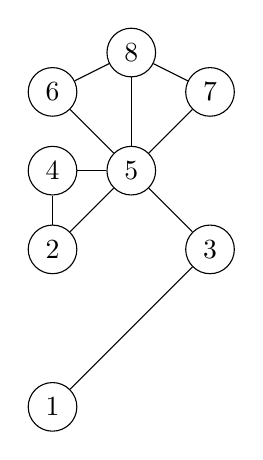
\begin{tikzpicture}
	\node (1) at (0,0) [shape=circle, draw] {1};
	\node (2) at (0,2) [shape=circle, draw] {2};
	\node (3) at (2,2) [shape=circle, draw] {3};
	\node (4) at (0,3) [shape=circle, draw] {4};
	\node (5) at (1,3) [shape=circle, draw] {5};
	\node (6) at (0,4) [shape=circle, draw] {6};
	\node (7) at (2,4) [shape=circle, draw] {7};
	\node (8) at (1,4.5) [shape=circle, draw] {8};


	\path 	[-]	(1) 	edge 	(3)
			(2)	edge	(4)
				edge 	(5)
			(3)	edge	(5)
			(4)	edge	(5)
			(5)	edge	(6)
				edge 	(7)
				edge 	(8)
			(6)	edge	(8)
			(7)	edge	(8);
\end{tikzpicture}
\end{center}

\item Given a $3\times 3\times 3$ lattice (like a cube) can you make a path for each of the following conditions
  that visits every vertex exactly once?  An image of a lattice is shown below (the wireframe cube surrounding the
  lattice is not a part of the problem).

\begin{enumerate}
	\item The walk must start one of the corners or the center of a face.
	\item The walk must start at an edge but not a corner.
\end{enumerate}

\begin{center}
	\includegraphics[width=.4\textwidth]{c1.png}
\end{center}

\item During CS 20 staff meeting, each of five TFs fell asleep exactly twice.  For each pair of these teaching fellows,
  there was some moment when both were sleeping simultaneously.  Prove that, at some moment, some three of them were sleeping simultaneously.
  \footnote{Adapted from USAMO 1986 Problem 2} \vspace{6 pt} \\
  \emph{Hints:}
  \begin{itemize}
    \item Consider a graph with 10 vertices, one for each time a TF slept.  Draw edges between two vertices if those two naps overlapped.
    \item What is the significance of a cycle in this graph?
  \end{itemize}

\end{enumerate}
\end{document}
